% =============================================================================
\subsection{Training dynamics: SSL and FOMAML losses}
\label{sec:training-curves}
% =============================================================================

The two unsupervised stages introduced in
Section~\ref{sec:tier0}~(SSL) and
Section~\ref{sec:tier1}~(FOMAML) produce the loss
trajectories in
Figure~\ref{fig:training-curves}.  The left panel
shows SSL reconstruction loss on the 4-scene~Sionna
mix: both train and val drop by an order of magnitude
in the first $\sim$10 epochs and then settle around
$1.0 \times 10^{-2}$ for the remaining 80, with an
isolated val spike near epoch~85 that recovers
immediately --- so the encoder is effectively done by
epoch~20.  The right panel shows the FOMAML outer
loop over 100 episodes with 10 train environments
sampled $n_{\text{way}}{=}4$ per meta-batch.  The
thick curve is the overall query loss (the value
FOMAML backpropagates); it drops from $0.83$ at
epoch~1 to $0.04$ at epoch~40, then oscillates
between $0.04$ and $0.10$ for the rest of training
--- composition noise from random meta-batches, not
instability.  The thin dotted curves are the
per-task support loss at the final inner step, one
line per environment: all 10 tasks converge
monotonically from a mean of $0.68$ to $0.03$ --- a
$22\times$ reduction with no failed environment.
The persistent gap between the support loss and
the query loss is the inner-loop gain, which stays
$\sim\!2\times$ even at epoch~100 and confirms the
inner adaptation is doing real work throughout
training.

\begin{figure}[t]
  \centering
  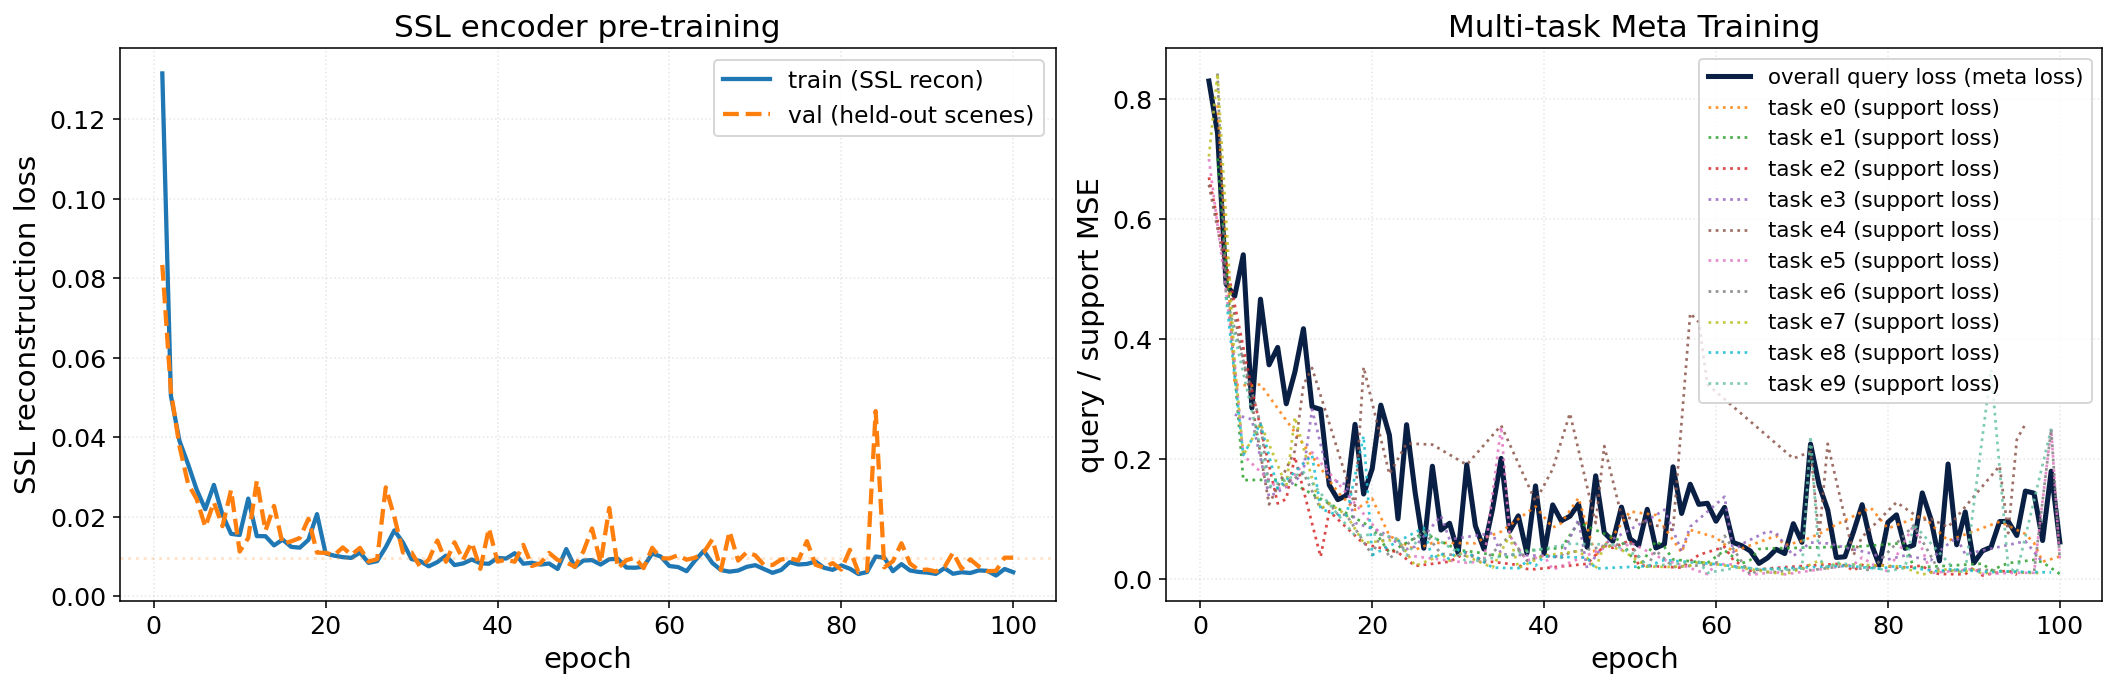
\includegraphics[width=\linewidth]{figures/ssl_vs_meta_with_taskloss_100ep.png}
  \caption{Training-time loss curves. \textbf{Left:}
  SSL reconstruction loss on the 4-scene~Sionna mix
  over 100 epochs (train solid, val dotted).
  \textbf{Right:} FOMAML outer loop over 100
  episodes.  Thick dark-navy: overall query loss
  (meta loss) averaged across the meta-batch.  Thin
  dotted (one color per env): per-task support loss
  at the final inner step.  Both panels share the
  x-axis (``epoch'').}
  \label{fig:training-curves}
\end{figure}
